\begin{appendices}

\chapter{Material für Nutzerstudie}
\label{appendix:study_material}
\todo{Fragebögen einfügen.}

\begin{figure}[hbt]
    \centering
    \framebox{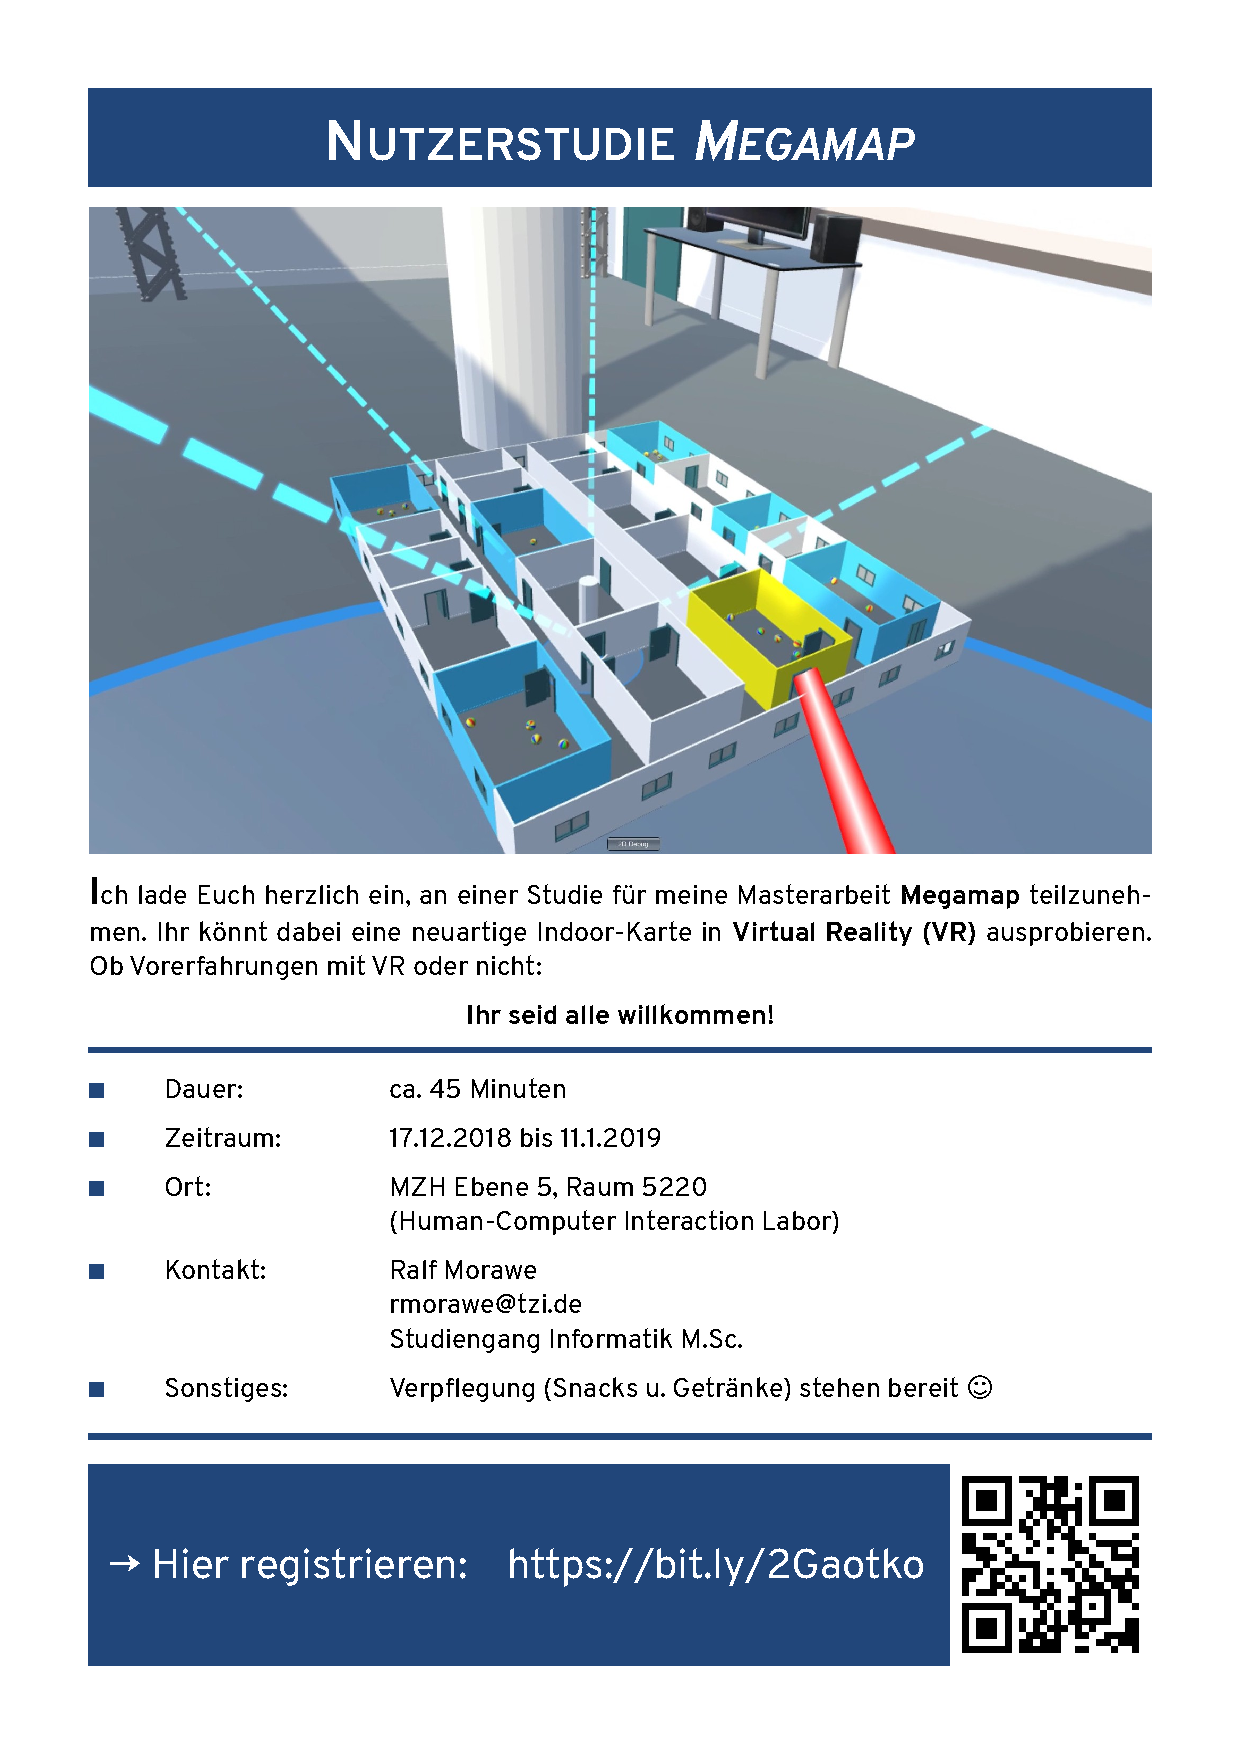
\includegraphics[width=0.725\linewidth]{appendix/study_flyer}}
    \caption{Flyer für Nutzerstudie.}
\end{figure}

\begin{figure}[hbt]
    \centering
    \begin{subfigure}{0.6\linewidth}
        \framebox[\width]{
\includegraphics[page=1, width=\linewidth]{appendix/study_infos}}
    \end{subfigure}

    \begin{subfigure}{0.6\linewidth}
        \framebox[\width]{
\includegraphics[page=2, trim={0, 13cm, 0, 0}, clip, width=\linewidth]{appendix/study_infos}}%
    \end{subfigure}%
    \caption{Informationsbogen für Probanden.}
\end{figure}

\begin{figure}[hbt]
    \centering
    \framebox{
\includegraphics[width=0.725\linewidth]{appendix/Zustimmung-Studienteilnahme}}
    \caption{Zustimmungsbogen für Probanden.}
\end{figure}

\end{appendices}
